\chapter{Introducción}
\label{chap:introduccion}


\section{Los Desechos Espaciales}

El comienzo de la era satelital en el a\~no 1957 con el sat\'elite ruso Sputnik signific\'o la conquiste de un nuevo espacio y un cambio de paradigma en lo que respecta a las tecnolog\'ias para las comunicaciones, los estudios de nuestro planeta y el sistema solar, las formas de navegar y geoposicionarse y el intercambio de informaci\'on. Desde entonces el ambiente espacial cada vez suma m\'as colonos.\\

Las experiencias de las primeras misiones aportaron mucho conocimiento de este entorno con caracter\'isticas muy distintas a las de la superficie de la Tierra y permitieron ir mejorando las t\'ecnicas y los materiales para que los sat\'elites cumplieran sus objetivos sin mayores inconvenientes.\\
Sin embargo, un hecho poco predicho o abordado empez\'o a ocupar prioridad en las dos \'ultimas d\'ecadas: los {\it{desechos espaciales}}.\\

{\bf{Definici\'on:}}{\it{ Son Desechos Espaciales todos los objetos construidos por el hombre, incluyendo fragmentos o partes de los mismos, que orbtian la Tierra o reingresan a la atm\'osfera y no son funcionales, es decir, han perdido su capacidad operativa.}} \citep{iadcguide}\\

La ocupaci\'on del espacio parec\'ia ilimitada, y los primeros a\~nos no se ten\'ian consideraciones respecto a los objetos que all\'i se depositaban, o se desprend\'ian de los cohetes y las misiones. Pero con el correr del tiempo, ciertas regiones cobraron inter\' es estrat\'egico, y la superpoblaci\' on en dichas zonas no tard\'o en mostrar complicaciones.\\

La primera colisi\'on confirmada y claramente registrada entre dos objetos catalogados ocurri\'o el 24 de Julio de 1996, cuando el sat\'elite franc\'es Cerise (95-033B) fue embestido por un fagmento (86-019RF), remanente de la explosi\'on de la \'ultima etapa del Ariane-1 H-10, que hab\'ia explotado el 13 de noviembre de 1986; nueve meses despu\'es de inyectar en \'orbita al sat\'elite SPOT-1. La reconstrucci\'on de la situaci\'on luego de la colisi\'on, coincide plenamente con una p\'erida de la actitud del Cerise que fue registrada en los datos hist\'oricos abordo. \citep{KlinkradChapter8}\\

Existen distintos abordajes o estudios respecto a la problem\'atica de los desechos espaciales. La \ac{NASA} propone una clasificaci\'on general seg\'un sean estudios de: modelado, rastreo, protecci\'on, mitigaci\'on, remediaci\'on o reingreso.\\
\begin{itemize}
%\setlength{\itemsep}{0pt}
\item {\bf{Modelado:}} Consiste en el desarrollo y la actualizaci\'on de los modelos orbitales de los desechos, para describir y caracterizar el ambiente actual y la proyecci\'on futura.\\
\item {\bf{Rastreo:}} Mediciones que se hacen con radares y telescopios \'opticos desde tierra, y tambi\'en con telescopios espaciales.\\
\item {\bf{Protecci\'on:}} Estudios hechos en impactos de alta velocidad para el desarrollo de nuevos materiales y dise\~nos que ofrezcan una mayor protecci\'on.\\
\item {\bf{Mitigaci\'on:}} Planifiaci\'on de estrategias para reducir la generaci\'on de nuevos desechos. Generaci\'on de documentaci\'on  de buenas pr\'acticas, est\'andares y promoci\'on de acuerdos internacionales.\\
\item {\bf{Remediaci\'on:}} Dise\~no de misiones que se encarguen de reducir el n\'umero de objetos inactivos en \'orbita.\\
\item {\bf{Reingreso:}} Identificaci\'on de los reingresos no controlados, para hacer an\'alisis sobre las zonas de posibles impactos en Tierra y la planificaci\'on de reingresos controlados.\\
\end{itemize}

Organismos como el Centro Principal de Inteligencia Espacial Ruso, el Departamento de Defensa Norteamericano, la NASA y la \ac{ESA}, han desarrollado tanto modelos de evoluci\'on como de ingenier\'ia, y mantienen cat\'alogos actualizados con las trayectorias de aquellos objetos cuyo tama\~no permite detectarlos con instrumentos de rastreo en Tierra.\\

Los modelos de evoluci\'on muestran la configuraci\'on actual y proyecciones de configuraciones futuras del ambiente espacial incluyendo todos los objetos que orbitan la Tierra.\\

Los modelos de ingenier\'ia se enfocan en distintas pruebas de laboratorio o de misiones espec\'ificas en \'orbita, que testean la respuesta de los materiales cuando se exponen a impactos con fragmentos de distinto tipo, particularmente en aquellos de tama\~nos muy chicos pero que colisionan a velocidades del orden de diez kil\'ometros por segundo.\\

En este trabajo nos enfocamos en el an\'alisis de las situaciones de riesgo de colisi\'on, dentro del marco de la {\it{mitigaci\'on}}, y particularmente para las misiones y los desechos que se ubican en las \'orbitas bajas \ac{LEO}.\\

\subsection*{El entorno de los Desechos Espaciales}
Seg\'un los informes de la Agencia Espacial Europea \citep{esaSD}, desde 1957 hasta la actualidad, 5250 lanzamientos han poblado el ambiente espacial con casi 23000 objetos de los cuales, s\'olo cerca de 1200 son sat\'elites operativos.\\

De a acuerdo a una publicaci\'on de la \cite{ODQNum}, hasta el 04 de Julio de 2017, se contabilizan $18347$ objetos catalogados que orbitan la Tierra, Fig. \ref{fig:catxpais}. Clasificados seg\'un sean: plataformas, cohetes, desechos de misi\'on, desechos an\'omalos o desechos de fragmentaci\'on.\\

\begin{figure}[!h]
\centering
  \subfigure[Objetos en \'Orbita al 4 de Abril de 2007.]{
    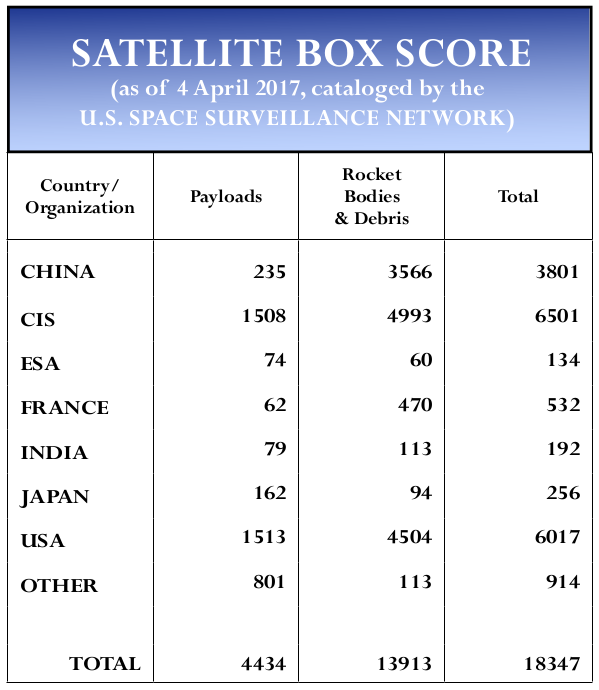
\includegraphics[width=0.35\columnwidth, keepaspectratio]{imagenes/catalogoXpais}
    \label{fig:catxpais}
  }
  \subfigure[Porcentaje de Objetos en \'Orbita seg\'un su clasificaci\'on.]{
    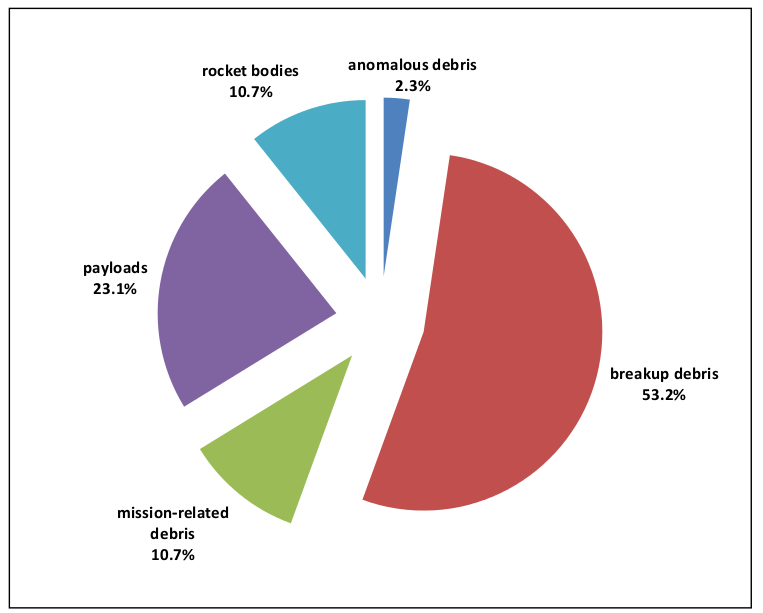
\includegraphics[width=0.5\columnwidth, keepaspectratio]{imagenes/clasificacion2016}
    \label{fig:catxtipo}
  }
  \caption[Objetos en \'Orbita]{Objetos que Orbitan la Tierra. Extra\'ido de \cite{ODQN}}
\end{figure}
Como puede apreciarse en la Fig. \ref{fig:catxtipo}, las plataformas de servicio o sat\'elites: {\it{payloads}}, representan el $23.1 \%$ pero si tenemos en cuenta s\'olo los sat\'elites operativos actualmente, el n\'umero se reduce casi al $7\%$ \\

La distribuci\'on de los sat\'elites y los  desechos que orbitan la Tierra no es homog\'enea. La relaci\'on entre la densidad de objetos y la altura a la que se encuentran, señala que existen regiones m\'as comprometidas.
Las \'orbitas bajas o \ac{LEO} con un rango de alturas entre los 600 y los 2000 kil\'ometros, son las m\'as superpobladas y contienen casi el 70 \% de todos los objetos catalogados. Ver figura \ref{fig:Dvsaltura}

\begin{figure}[!h]
  \centering
  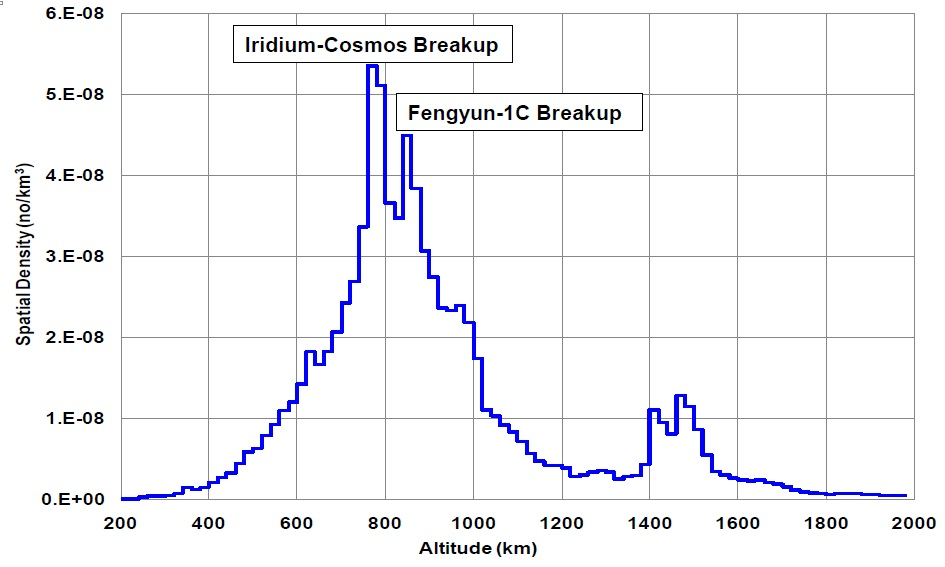
\includegraphics[width=0.75\textwidth]{imagenes/SDvsaltura2011}
  \caption[Distribuci\'on de objetos en funci\'on del semieje mayor.]{Distribuci\'on de objetos en funci\'on del semieje mayor. Adapatado de \citep{Klinkrad}}
  \label{fig:Dvsaltura}
\end{figure}

En un reporte t\'ecnico publicado por la NASA \citep{karacalioglu2016impact}, se eval\'uan las nuevas tendencias de la industria satelital y se analiza el futuro panorama del entorno espacial en las \'orbitas bajas, en funci\'on de los lanzamientos planificados y las misiones anunciadas, Fig. \ref{fig:satxlanz}.\\

\begin{figure}[!h]
  \centering
  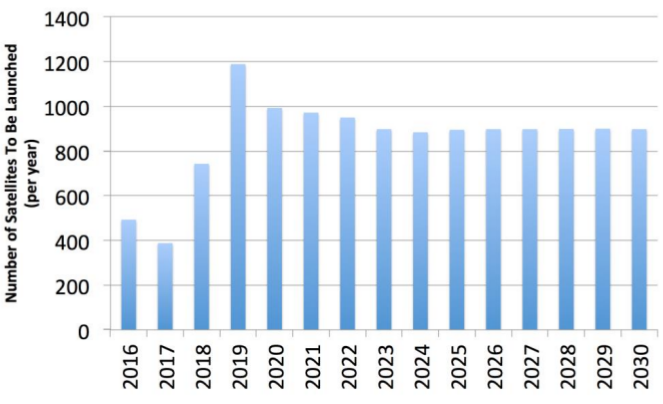
\includegraphics[width=0.8\textwidth]{imagenes/satelxlanz}
  \caption[Proyecci\'on de Sat\'elites 2016-2030]{Proyecci\'on de Sat\'elites 2016-2030. Extra\'ido de \citep{karacalioglu2016impact}}
  \label{fig:satxlanz}
\end{figure}

En los \'ultmos a\~nos se ha incrementado el n\'umero de agencias o empresas que se de dedican al desarrollo espacial. El nuevo paradigma de constelaciones de peque\~nos sat\'elites, sistemas distribuidos o arquitecturas fragmentadas en reemplazo de los grandes y costosos sat\'elites tradicionales, ha permitido la democratizaci\'on del espacio, facilit\'andole el acceso a m\'as agencias y empresas.\\ 
Un claro ejemplo son las constelaciones para comunicaciones anunciadas por OneWeb y SpaceX, que proyectan lanzar del orden de 600 sat\'elites cada una para fines del 2019.\\

Estos sat\'elites incrementan la superpoblaci\'on de objetos en \'orbita durante su vida \'util y dependiendo de sus caracter\'isticas, pueden permanecer en \'orbita inactivos por m\'as de 20 a\~nos si no se toman medidas de reingreso una vez finalizada su misi\'on.\\
A su vez, aunque ya existen modelos experimentales y en desarrollo en lo que respecta a recuperar partes de los lanzadores, cada lanzamiento injecta en \'orbita fragmentos del cohete {\it{rocket bodies}} Fig. \ref{fig:rocketbodies}.\\

\begin{figure}[!h]
  \centering
  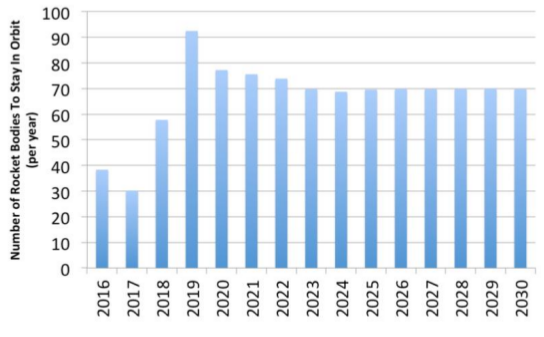
\includegraphics[width=0.8\textwidth]{imagenes/rocketbodies}
  \caption[Fragmentos de Cohetes 2016-2030]{Fragmentos de Cohetes que permanecer\'an en \'orbita en el periodo 2016-2030. Extra\'ido de \cite{karacalioglu2016impact}}
  \label{fig:rocketbodies}
\end{figure}

\section{El Riesgo de Colisi\'on}

La primera colisi\'on catastr\'ofica que se registra, ocurri\'o entre el sat\'elite ruso KOSMOS \- 2251 que hab\'ia quedado fuera de servicio y el sat\'elite operativo IRIDUM33 de la constelaci\'on de IRIDIUM en el a\~no 2009.\\
El evento ocurri\'o a 790 kil\'ometros de altura y gener\'o m\'as de 2500 fragmentos, 500 de ellos a\'un permanecen en \'obita. Este panorama, marc\'o la materializaci\'on de una situaci\'on que se preve\'ia que pod\'ia ocurrir y ofici\'o de catalizador de los estudios vinculados a la predicci\'on, an\'alisis y mitigaci\'on del riesgo de colisi\'on.\\

\textcolor{red}{Transformar imagen en TABLA}
\begin{figure}[!h]
  \centering
  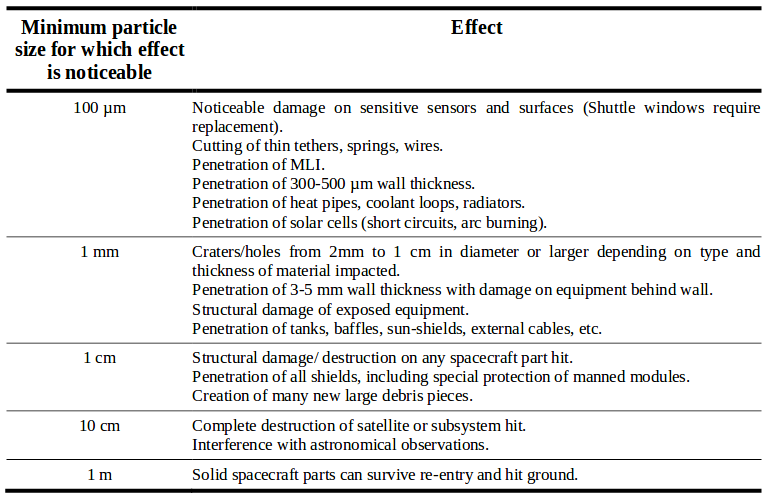
\includegraphics[width=0.9\textwidth]{imagenes/danioxtamanio}
  \caption[Efecto de impacto seg\'un tama\~no del desecho.]{Efecto de impacto seg\'un tama\~no del desecho.Extra\'ido de IADC 08-03 version2.1 Abril 2013 }
  \label{fig:causadesechos}
\end{figure}


De los distintos modelos y de las descripciones del ambiente espacial a trav\'es de los a\~nos, se distingue claramente como aumenta el n\'umero de desechos cuando ocurren colisiones significativas. En sentido inverso, se prevee que a partir del incremento de objetos, en particular en las \'orbitas bajas, aumenten las colisiones, convirti\'endose las mismas, en las principales fuentes de generaci\'on de desechos.\\ 

Como puede apreciarse en la Fig. \ref{fig:causadesechos} el porcentaje del remanente de desechos producto de rupturas debido a diferentes causas, fue modific\'andose en los \'ultimos a\~nos. Las distintas pol\'itcas de mitigaci\'on en relaci\'on a explosiones intencionales, el remanente de combustibles, un enfoque m\'as profundo en el tratamiento de las bater\'ias y la protecci\'on de los materiales frente a impactos, han reducido el n\'umero de desechos producto de explosiones intencionales, explosiones generadas por los combustibles, las fallas de las bater\'ias y  las causas desconcidas. Mientras que los desechos generados por colisiones han aumentado.\\

% \begin{figure}[!h]
%   \centering
%   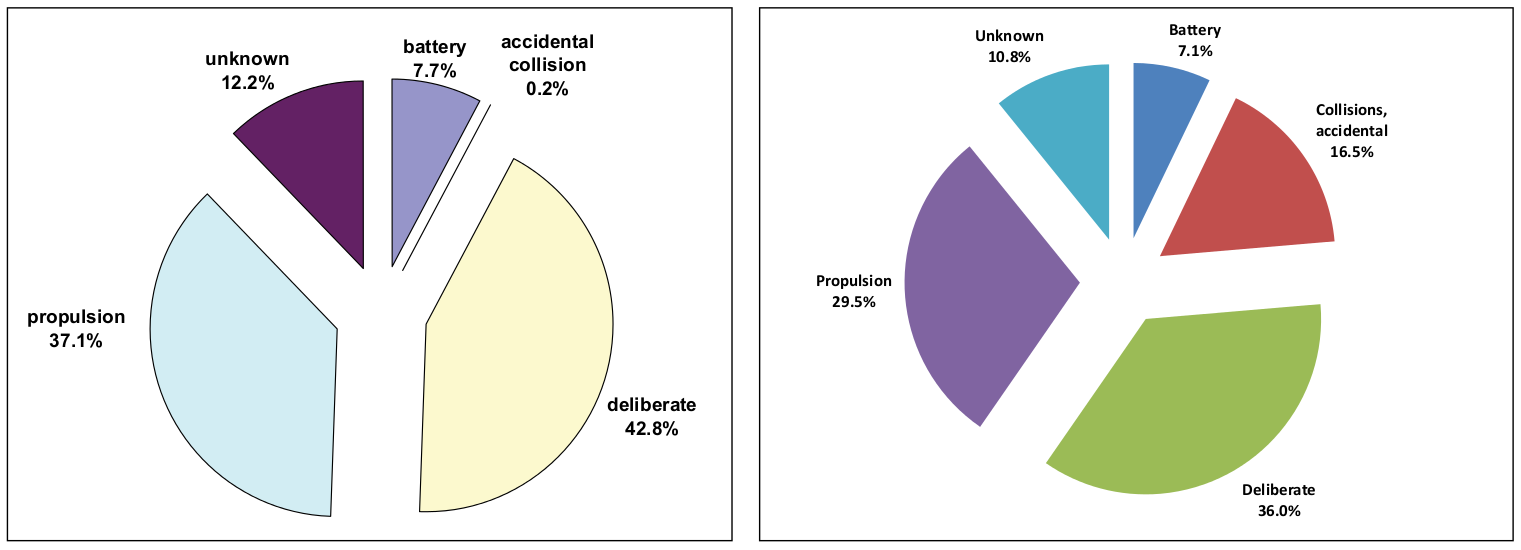
\includegraphics[width=0.9\textwidth]{imagenes/breakupsQNews}
%   \caption[Evoluci\'on de las causas de la generaci\'on de Desechos]{Evoluci\'on de las causas de la generaci\'on de Desechos entre 2007 y 2016. Extra\'ido de \citep{ODQNum}}
%   \label{fig:causadesechos}
% \end{figure}

Conclusiones similares se desprenden del estudio de \citep{karacalioglu2016impact}, cuyas simulaciones futuras se\~nalan que en los pr\'oximos a\~nos ser\'an las colisiones las que mayor n\'umero de desechos aporten al total de objetos que orbitan la Tierra en las \'orbitas bajas Fig. \ref{fig:debriscollision}\\

% \begin{figure}[!h]
%   \centering
%   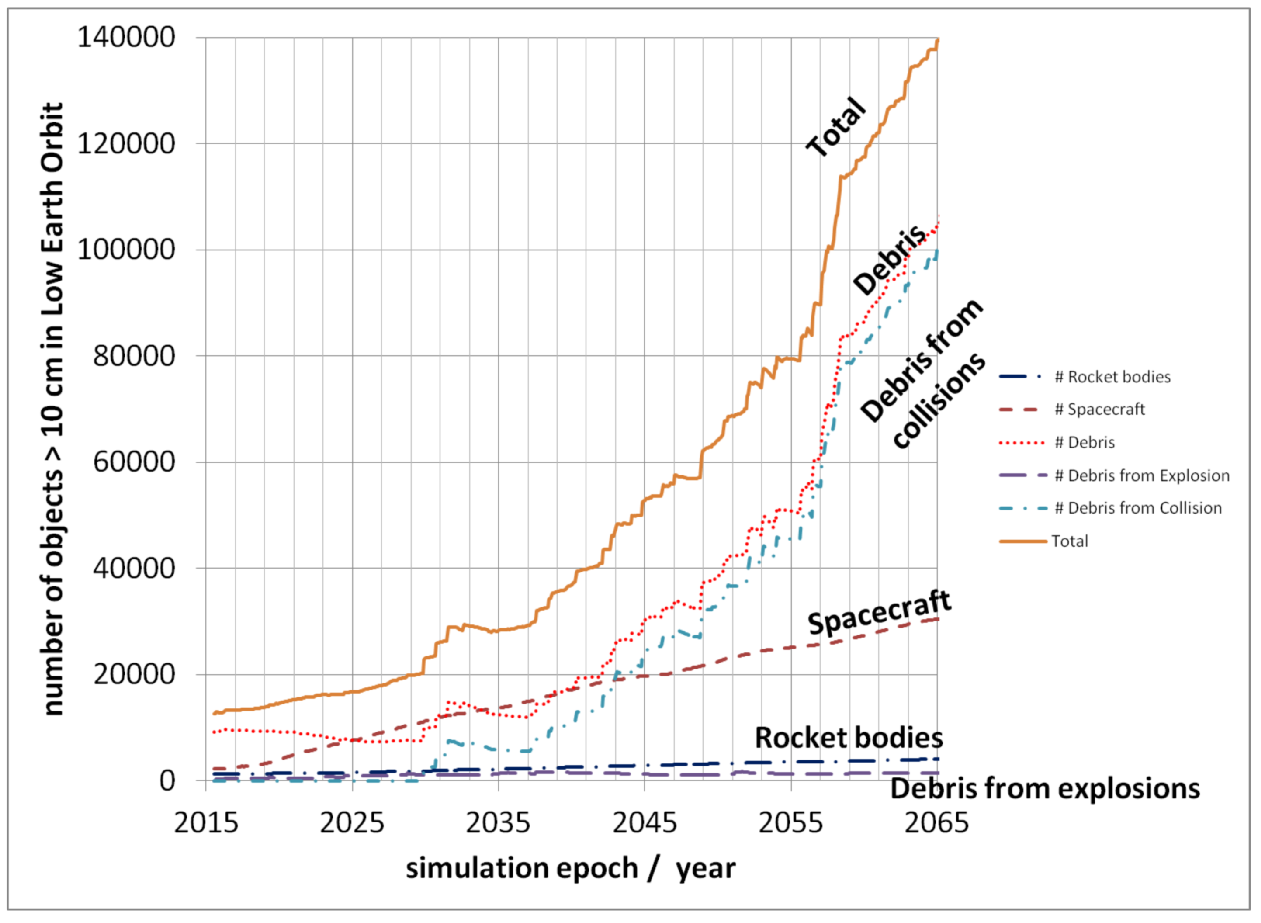
\includegraphics[width=0.7\textwidth]{imagenes/debriscollision}
%   \caption[N\'umero de Desechos en las \'orbitas LEO desde 2015 al 2065]{N\'umero de Desechos en las \'orbitas LEO desde 2015 al 2065. Extra\'ido de \citep{karacalioglu2016impact}}
%   \label{fig:debriscollision}
% \end{figure}

Ya en 1978  estudios predictivos hechos por D. Kessler y Cour-Palais
 \cite{kessler0}, anunciaban el riesgo del efecto en cascada que podr\'ian producir las colisiones, aumentando los desechos en un camino catastr\'ofico sin fin y mostrando que los desechos generados por colisiones superar\'ian los impactos por meteoritos.\\

 \subsubsection*{El estudio del riesgo de colisi\'on}

Un an\'alisis completo del Riesgo de Colisi\'on Fig. \ref{fig:estudiocolision}, abarca:

\begin{itemize}
\setlength{\itemsep}{0pt}
\item Identificar las situaciones de encuentro.
\item Analizar la situaci\'on del encuentro.
\item Ejecutar maniobras de mitigaci\'on del riesgo si fuera necesario.
\item Iterar el proceso con minuciocidad para no ofrecer soluciones moment\'aneas que generen nuevos riesgos de colisi\'on.
\end{itemize}

{\bf{Identificaci\'on de las situaciones de encuentro:}}\\
A partir de los datos generados por las redes de rastreo (Ver \ref{subsec:redes}), se propagan las trayectorias orbitales y, bajo ciertos criterios definidos previamente, se detectan los acercamientos no deseados. En esta idea subyace la definici\'on de {\it{Encuentro}}.\\
Son pocos los organismos y agencias capaces de realizar este procedimiento, incorporando a sus predicciones todos los objetos catalogados y/o rastreados.\\
En un formato m\'as simplificado, el inter\'es se enfoca en una misi\'on en particular y se desarrollan filtros, para procesar encuentros analizando una menor cantidad de objetos.\\


{\bf{An\'alisis de la situaci\'on del encuentro: }}\\
El mismo consiste en estudiar el encuentro con mayor profundidad y detalle, sumando informaci\'on m\'as confiable en la determinaci\'on orbital, y calculando par\'armetros estad\'isticos, como la Probabilidad de Colisi\'on (PoC).\\
A medida que se aproxima la fecha en la que se predice el encuentro, se tiene mejor conocimiento de la \'orbita de los objetos involucrados, pero menor tiempo de reacci\'on en la toma de decisiones. Es decir, en el an\'alisis del encuentro se busca un balance entre los tiempos que conlleve el estudio para alcanzar la confiabilidad necesaria, y el margen que se requiere para, por ejemplo, planificar una maniobra.\\
En este item en particular se enfoca este trabajo.\\

{\bf{Realizaci\'on de una maniobra:}}\\
Si la situaci\'on lo ameritara, la \'unica manera de evitar una colisi\'on es la {\bf{realizaci\'on de una maniobra}}, conocidas como Maniobras de Mitigaci\'on de Riesgo (RMM). No obstante, modificar la trayectoria de un objeto, siempre presupone una evaluaci\'on a priori de que no vaya a producirse una colisi\'on. De manera, que en este punto, se realizan propagaciones con las posiciones estimadas durate y luego de la maniobra, y se itera el proceso para estas nuevas posiciones contra el cat\'alogo de objetos.\\ 


% La exitosa Misi\'on SAC-D/AQUARIUS de la CONAE en convenio con la \ac{NASA}, contabiliz\'o del orden de cinco RMM registradas, a lo largo de su vida \'util [10]. Mientras que la \ac{ISS} realiza casi una maniobra de riesgo de colisi\'on por año, dada su envergadura.\\

% \begin{figure}[!h]
%   \centering
%   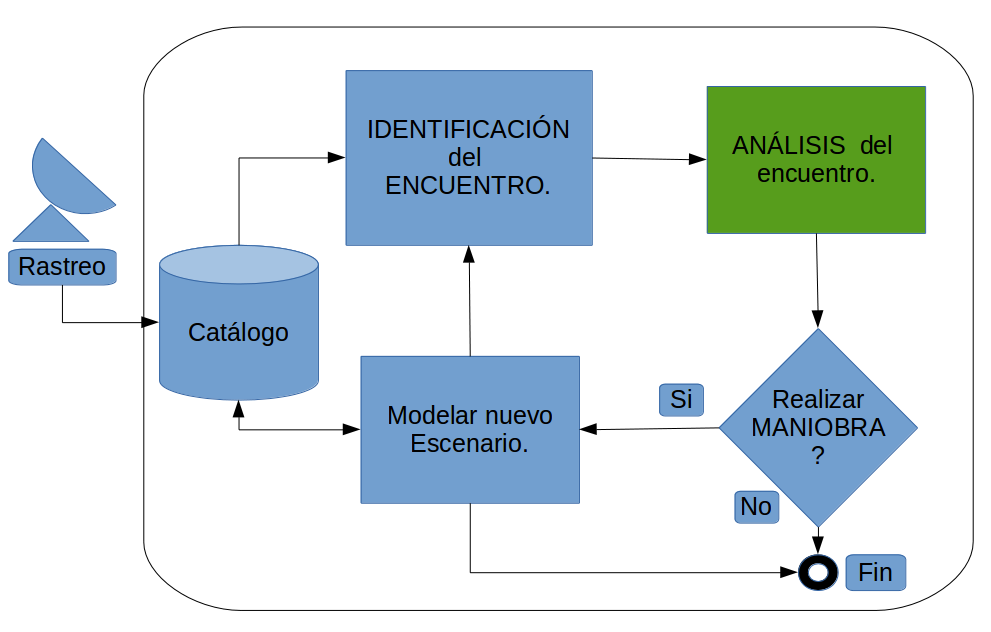
\includegraphics[width=0.6\textwidth]{imagenes/estudiocolision}
%   \caption[Estudio de Colisi\'on]{Esquema de alto nivel de los procesos en un estudio completo de riesgos de colisi\'on. (Se indica en color verde, la etapa que se desarrolla en este trabajo.)}
%   \label{fig:estudiocolision}
% \end{figure}


% CONCEPTO DE MIDDLE MAN.\\
% CONCEPTO DE COLLABORATIVE WORK ENVIRONMENT. (close loop process)

\subsection*{Rastreo y cat\'alogos}\label{subsec:redes}

En los catálogos actuales se registran objetos mayores a los 10 cm en las regiones LEO monitoreadas con radares, y mayores a 1 m en las órbitas GEO observadas con telescopios ópticos.\\
 
La entidad militar US Strategic Command (USSTRATCOM) de EE.UU mantiene un catálogo con 18347 objetos conocidos (al 4 de Abril de 2016). Para su construcci\'on y mantenimiento, utiliza la Space Surveillance Network (SSN), Fig.\ref{fig:usnet}  que posee m\'as de 20 sensores civiles y militares a lo largo de todo el mundo.\\

\begin{figure}[!h]
  \centering
  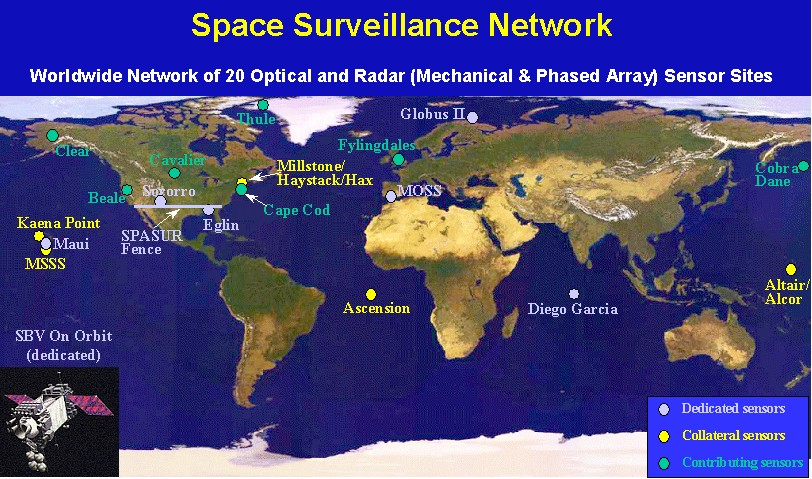
\includegraphics[width=0.9\textwidth]{imagenes/SpSNet}
  \caption[USSTRATCOM - SSN]{US. Strategic Command Space Surveillance Network. Extra\'ido de https://en.wikipedia.org/wiki/United\_States\_Space\_Surveillance\_Network}
  \label{fig:usnet}
\end{figure}

Rusia es la única nación, aparte de EE.UU, que cuenta con un sistema de rastreo que le proporciona una base de datos de objetos espaciales artificiales significativa y actualizada.\\
A su vez, independiente del gobierno Ruso, el KIAM1 promueve la red internacional: International Scientific Optical Network (ISON), que ofrece uno de los programas coordinados de monitoreo de desechos más importante.
La red cuenta con 30 telescopios en el rango de 0.5 a 2.6 m de diámetro, repartidos en 20 observatorios de 8 países en todo el mundo.\\

Por su parte, la ESA inició programas de monitoreo hace ya varios años.\\
En la actualidad las investigaciones están predominantemente realizadas por las agencias espaciales: ASI (Italia), BSNC (UK), CNES (Francia), y DLR (Alemania), con el apoyo de la industria, institutos de investigación y universidades. En los últimos 10 años han estado trabajando en forma coordinada para implementar un Sistema Europeo de Vigilancia Espacial.
A tal fin cuentan con varios telescopios ópticos como el Zeiss de 1 m de Tenerife, el Schimdt y Tarot en Francia, o los sensores PIMS (Passive Imaging Sensors) del Reino Unido, y con importantes radares, como el TIRA (Tracking and Imaging Radar) en Alemania, o los más modernos EISCAT Y EICAT 3D (European Incoherent Scatter Radar) que logran detecciones de objetos del orden de los centímetros a distancias de 800 km.


% \begin{verbatim}
%  Settecerri, T. J et al – “Haystack measurements of the orbital debris environment” – Advances in Space Research 1999.
% Mehrholz, et al – “Beam-park experiments at FGAN” –  AdSpR 2004.
% Igor Molotov, et al – “Faint High Orbital Debris Observations with ISON Optical Network” – 
% Proceedings of the Advanced Moui Optical and Space
% \end{verbatim}



\section{Las Regulaciones Nacionales e Internacionales}

Dado el car\'acter global de esta problem\'atica, distintas naciones y agencias internacionales con gran desarrollo y actividad espacial, se han estado organizado en la b\'usqueda de acuerdos y buenas pr\'acticas. Entre los organismos que coordinan las recomendaciones, se encuentran:\\

\begin{itemize}
\item COPUOS: Committee of the Peacefull Uses of Outer Space \ac{ONU}
\item IADC: Inter-Agency Space Debris Coordination Committee
\item CCSDS: Consultative Committee for Space Data Systems
\end{itemize}

La NASA fue la primera en adoptar un set de lineamientos para la mitigaci\'on de los desechos espaciales en 1995, que fueron posteriormente incorporados por el gobierno de EE.UU en 1997.\\
En el a\~no 2002 el IADC conformado por diez pa\'ises y la ESA, elabor\'o un nuevo conjunto de lineamientos.
Finalmente en 2007 el subcomit\'e cient\'ifico y tecnol\'ogico del COPUOS aun\'o los esfuerzos y reuni\'o todos los trabajos previos, logrando un consenso en los lineamientos definitivos promulgados por la ONU en 2008 \citep{nasaprogramme}.\\

En lo que respecta a los l\'imites de este trabajo, podemos citar las siguientes Normas, Recomendaciones y Legislaci\'on:\\

\begin{itemize}
\item {\small{Convenio sobre Responsabilidad Internacional por da\~nos causados por objetos espaciales. ONU - (29-03-72)}}
\item {\small{Ley 23.335 (19-08-86) - Arg. Suscribe al Convenio de ONU.}}
\item {\small{Space Debris Mitigation Guidelines - IADC}}
\item {\small{ISO 24113:2011 {\it{Space Debris mitigation requirements}}}}
\item {\small{ISO/TR 16158:2013 {\it{Space Systems - Avoiding collision with orbiting objects}}}}
\item {\small{ISO 19389:2014 {\it{Space data and information transfer Systems}}}}

\end{itemize}

\section{Antecedentes}
En este contexto, ya existen claros antecedentes que abordan la problem\'atica con sus respectivos soportes inform\'aticos. (ver tabla \ref{tab:sisal})
\begin{table}[!h]
\centering
\begin{tabular}{|l|p{5cm}|p{6cm}|}
\hline
Herramienta & Descripci\'on & Proveedor/Agencia\\
\hline
{\bf{CARA}} & {\it{Conjunction Assessment Risk Analysis}} & NASA Robotic Conjunction Assessment Risk Analysis group, en convenio con la empresa a.i. solutions, Inc.\\
\hline
{\bf{SOCRATES}} & {\it{Satellite Orbital Conjuction Reports Assessing Threatening Encounters in Space}}, servicio web v\'ia Celestrack.com & CSSI (Center for Space Standards \& Innovation) de la agencia AGI: Analytical Graphics, Inc.\\
\hline
{\bf{CRASS}} & {\it{Collision Risk Assessment tool}} & Desarrollado por la
empresa GMV, que presta servicios al Centro Europeo de Operaciones
Espaciales (ESOC) - Darmstadt, Alemania. \cite{alarconRodriguez}\\
\hline
{\bf{CAESAR}} & {\it{Conjuction Analysis and Evaluation Service, Alerts and Recommendations}} & Agencia francesa CNES, que utiliza como soporte el Software JAC {\it{Java for Assessment of Conjunctions}}. \cite{laporte}\\
%\hline
%closeap - ant\'on & & ESA\\
\hline
{\bf{CRAMS}} & {\it{Collision Risk Assessment and Mitigation System}} & Canadian Space Agency (CSA). \cite{babiker}\\
\hline
\end{tabular}
\caption[Sistemas de Alerta]{Sistemas de Alertas de distintas Naciones y Agencias}
\label{tab:sisal}
\end{table}

\section{La Unidad de Desechos Espaciales de la CONAE}
De acuerdo con el Plan Nacional Espacial: {\bf{ Argentina en el Espacio 2004-2015}} [5], las misiones de la CONAE, fundamentalmente pensadas para observaci\'on de la Tierra, ocupan \'orbitas bajas de dise\~no estrat\'egico. Es decir, se ubican en regiones de mucha demanda y en consecuencia se encuentran expuestas a un alto riesgo de colisi\'on.\\
En nuestro pa\'is, compete a la Unidad de Desechos Espaciales de la Secretaria General de la CONAE; quien tiene la facultad de mantener las relaciones con los organismos internacionales, garantizar que se cumplan los distintos convenios y acuerdos a los que Argentina ha adherido, como por ejemplo el {\it{Convenio sobre la Responsabilidad Internacional por da\~nos causados por objetos espaciales}}, suscripto por la Rep\'ublica Argentina el 29 de marzo de 1972. (LEY N 23.335, sancionada: Julio 30 de 1986 - promulgada: Agosto 19 de 1986.1).\\
As\'i mismo, como miembro parte de la ONU, responde ante el COPUOS en materia de buenas pr\'acticas para la mitigaci\'on de la generaci\'on de desechos espaciales.\\

En la actualidad, las \'unicas naciones que cuentan con una red de rastreo con capacidad de detectar, rastrear y catalogar objetos son EE.UU y Rusia. De manera que Argentina planifica y ejecuta sus maniobras de riesgo (RMM) a partir de informaci\'on que le proveen servicios externos.\\

El an\'alisis de posible colisi\'on, es uno de los temas que se abordan con mayor delicadeza dentro del \'area espacial y dado el nivel de riesgo que implica, la CONAE contrata un servicio de asesoramiento y control para la planificaci\'on de las operaciones vinculadas al alerta por colisi\'on.\\
Ofrecer un servicio que reemplace al que utiliza actualmente en CONAE, es impensado y escapa por mucho a los alcances de este trabajo. No obstante, hemos desarrollado una herramienta que permite una clara caracterizaci\'on de la situaci\'on y un mayor conocimiento en el di\'alogo e intercambio de informaci\'on con los organismos y agencias que proveen el servicio y asesoramiento. As\'i mismo, se piensa como un planteo preliminar, con versatilidad para ser testeado, perfeccionado y ampliado a largo plazo.\\

\section{Planteo del Problema}

El desfavorable panorama futuro en materia de colisiones en \'orbita, conlleva a los centros de operaciones a incorporar procedimientos y soportes, para la gesti\'on, el an\'alisis y la prevenci\'on de las colisiones.\\
Dependiendo de las capacidades con las que las agencian cuentan, estos sistemas incluyen desde: redes o instrumentos espec\'ificos de rastreo propios, cat\'alogos completos de los objetos capaces de ser rastreados, sistemas de detecci\'on anticipada de acercamientos de riesgo, sistemas de an\'alisis de situaciones de riesgo alertadas por agentes externos o contrataci\'on de servicios externos que resuelven la totalidad del an\'alisis incluyendo la sugerencia de las maniobras pertinentes.\\

En este trabajo nos poroponemos ofrecer una herramienta enmcarcada en las dos \'ultimas situaciones mencionadas. Es decir, planteamos un modo operativo y un prototipo de software ...ARxCODE como soporte al estudio de los alertas. 
En pos de ofrecer un sistema que tenga la capacidad de procesar la informaci\'on de los mensajes de alerta externos (CDM) de JSpOC, y 
que permita adem\'as hacer un an\'alisis propio de la situacio\'on  

Llega un CDM que anuncia un riesgo de colisi\'on en el tiempo futuro $t_{ca}$, ¿qu\'e cosas me pregunto?

Preguntas:\\

\begin{enumerate}
 \item ¿Por qu\'e hablamos de probabilidad?
 \item ¿Con qu\'e error conozco la posici\'on de la Misi\'on para la \'epoca actual?\\
 \item ¿Con qu\'e error conozco la posici\'on del desecho para la \'epoca actual?\\
 \item ¿Con qu\'e error conozco la posici\'on de la Misi\'on para la \'epoca $t_{ca}$?\\
 \item ¿Con qu\'e error conozco la posici\'on del desecho para la \'epoca $t_{ca}$?\\
\end{enumerate}

\begin{enumerate}
 \item Error de la Misi\'on en la \'epoca actual: La posici\'on y velocidad se plasma en los productos que genera el CODS, a trav\'es de sus efem\'erides predichas y o precisas. El error asociado ... {\textcolor{red}{¿? : documento CODS y/o dato CDM}} - {\textcolor{red}{En nuestro trabajo utilizamos TLEs para su estimaci\'on y la generaci\'on de la matriz de covarianza.}} Como mostraremos m\'as adelante en el capítulo \ref{chap:metodologia}...\\
 \item Error del Desecho en la \'epoca actual: {\textcolor{red}{¿?:dato CDM}} - M\'etodo de Osweiler. Funci\'on de Ajuste a partir de la tendencia. (Validaci\'on utilizando datos CODS para comparar los resultados de la funci\'on de ajuste) - JSPoC no cuenta con info de maniobras planificadas.
 
\end{enumerate}

% \begin{figure}[!h]
% \centering
%   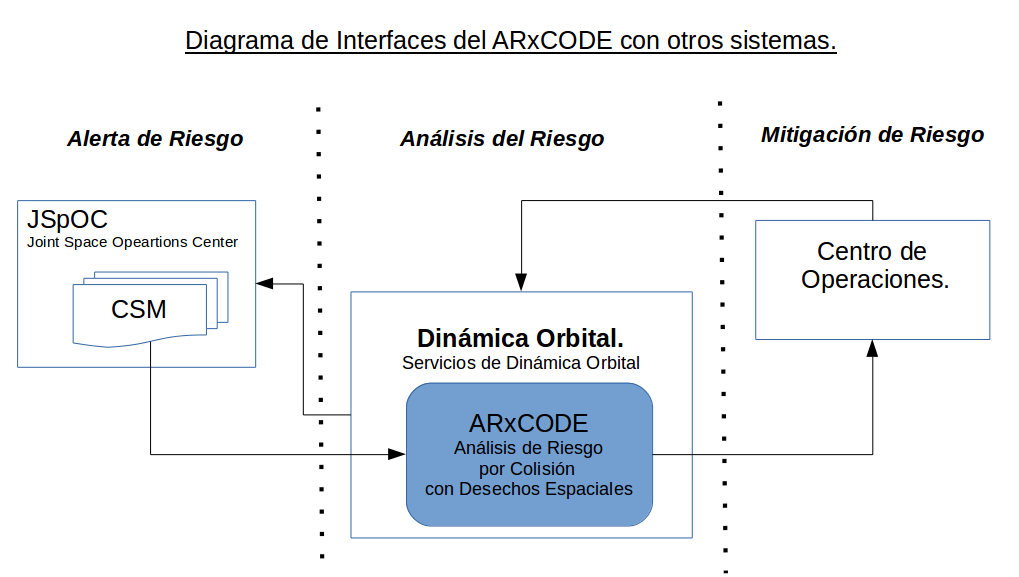
\includegraphics[width=0.7\textwidth]{imagenes/interfasessistemas}
% \end{figure}



\section{Objetivos}

% La herramienta ARxCODE para el An\'alisis de Riesgo por Colisi\'on con Desechos, que presentamos en esta tesis, consiste en un software que ser\'a montado sobre la estructura actual con la que cuenta el departamento de Din\'amica Orbital, y ser\'a utilizado por operadores del sector con amplios conocimientos del area.\\

% {\bf{Revisar este esquema para que cierre y vuelva a JSPoC}}
% El mismo oficiar\'a de intermediario entre los organismos internacionales que proveen los mensajes de alerta (CDM) y el operador de din\'amica orbital, quien se encargar\'a de procesar la informaci\'on con las facilidades que ARxCODE provee y generar los reportes necesarios para el intercambio de informaci\'on y la toma de decisiones.\\ 

\subsection*{Objetivo principal}
Diseñar un procedimiento operativo frente a situaciones de alerta por riesgo de posible
colisi\'on con desechos espaciales y desarrollar un prototipo de software: ARxCODE, que
mejore el c\'alculo de los par\'ametros de caracterizaci\'on del riesgo y facilite al analista la
toma de decisiones y/o el di\'alogo con los servicios de alerta externos.\\

\subsection*{Objetivos espec\'ificos}
\begin{itemize}
\item Automatizar la recepci\'on y gesti\'on de los mensajes de alertas (CDM) por posibles
colisiones, que se reciben de organismos internacionales de rastreo.
\item Desarrollar una t\'ecnica que mejore la determinaci\'on de la posici\'on del desecho es-
pacial.
\item Calcular la Probabilidad de Colisi\'on (PoC) para caracterizar la situaci\'on de encuen-
tro.
\item Desarrollar un prototipo de software (ARxCODE) para el procesamiento de la infor-
maci\'on, el manejo de las notificaciones, la visualizaci\'on del evento y la generaci\'on
de reportes.
\end{itemize}